\section{Output signals for different input signals}

To prove that the transmitter works correctly and to obtain performance results the output for different input signals was observed. Figure \ref{fig:alternating_data} shows the transient waveform for alternating data at the TX output for \unit[6]{UI}. The eye diagram over \unit[2940]{UI} for a PRBS15 data pattern is given by figure \ref{fig:eye_prbs15}. Equalization is disabled in this case, it would roughly half the vertical eye opening for \unit[6]{dB} of equalization at the first post cursor. The eye is not shown for \unit[10000]{UI} as I ran out of disk space and therefore the simulation stopped.\\
In figure \ref{fig:wc_eye} the eye for the worst case data pattern of the transmitter is drawn. Note that this pattern is different than the worst case data pattern of the channel as the eye at the Tx output is not determined by the channel characteristics but by the driving capabilities of the transmitter circuitry. Our design includes one post cursor and the main cursor. Therefore the eye opening is minimal when the post cursor and main cursor slices drive in opposite directions. The worst case is reached when the flipflops have to toggle their output in each cycle and therefore have to change the charge on the input capacitance of the following gates, generating a switching edge at their input. These also have to switch states and we get the worst possible input signal for our output drivers. Also the input flipflops separate the data in even and odd bit, so they toggle in each cycle for a bit sequence consisting of two equal bits in a row (00110011), which is our worst case pattern for the transmitter.

\begin{figure}[H]
  \centering
  \subfigure[with {\unit[6]{dB}} equalization]
  {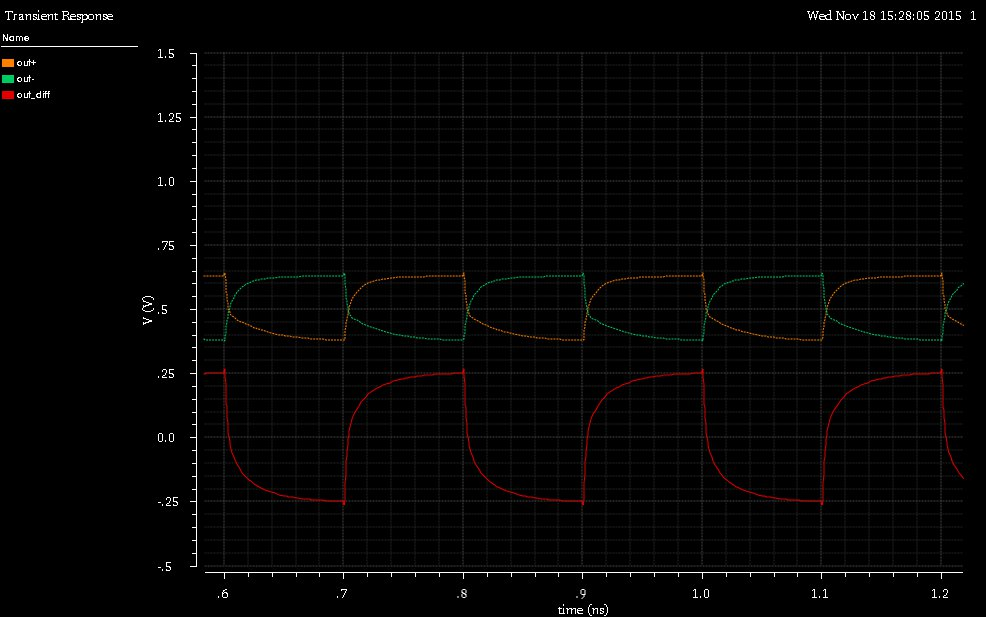
\includegraphics[scale=0.6]{img/alternating_data.jpg}}
  \subfigure[equalization turned off]
  {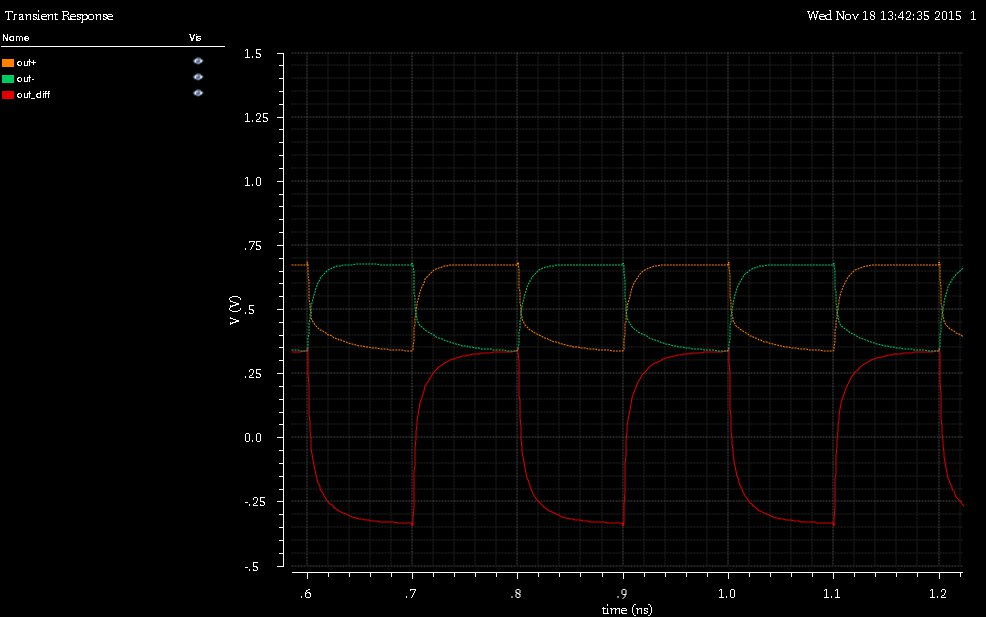
\includegraphics[scale=0.6]{img/alternating_data_no_eq.jpg}}
  \caption{Transmitter output for alternating data at the input}
  \label{fig:alternating_data}
\end{figure}

\begin{figure}[H]
  \centering
  {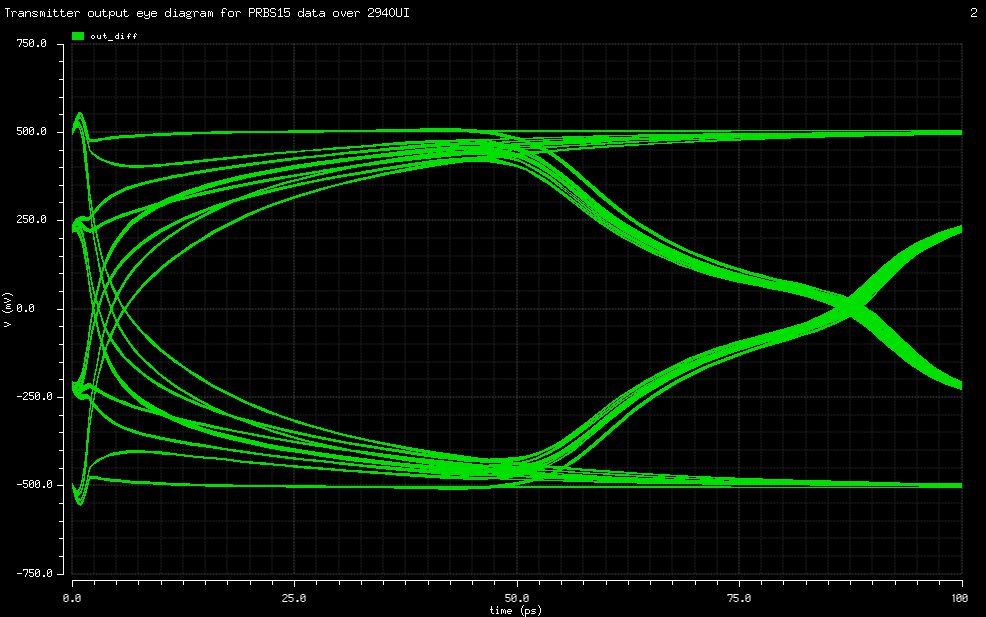
\includegraphics[scale=0.6]{img/prbs_eye.jpg}}
  \caption{Eye diagram over \unit[2940]{bits} for PRBS15 data pattern}
  \label{fig:eye_prbs15}
\end{figure}

\begin{figure}[H]
  \centering
  \subfigure[with {\unit[6]{dB}} equalization]
  {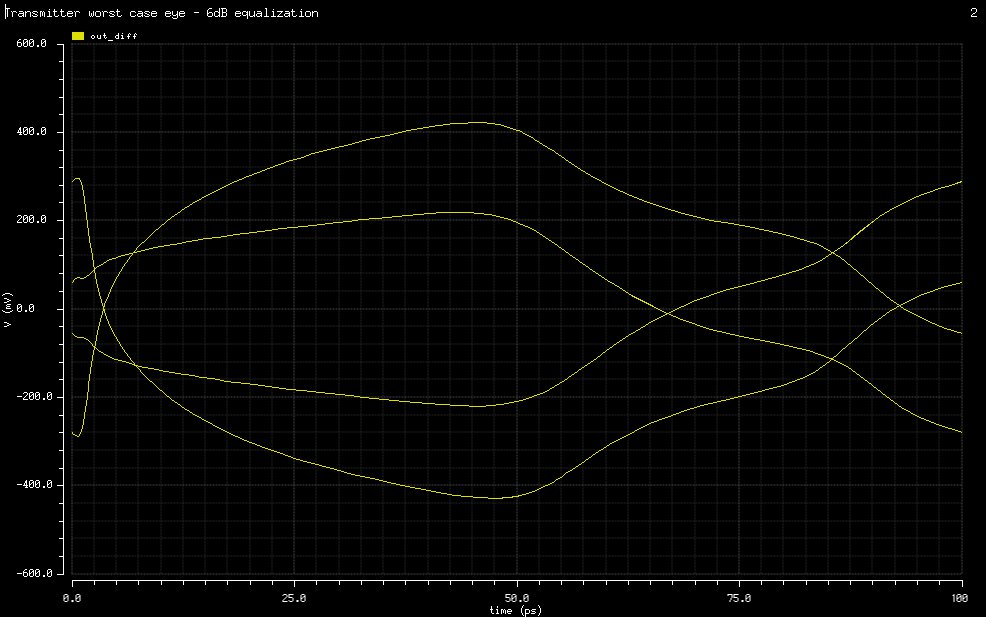
\includegraphics[scale=0.6]{img/wc_eye.jpg}}
  \subfigure[equalization turned off]
  {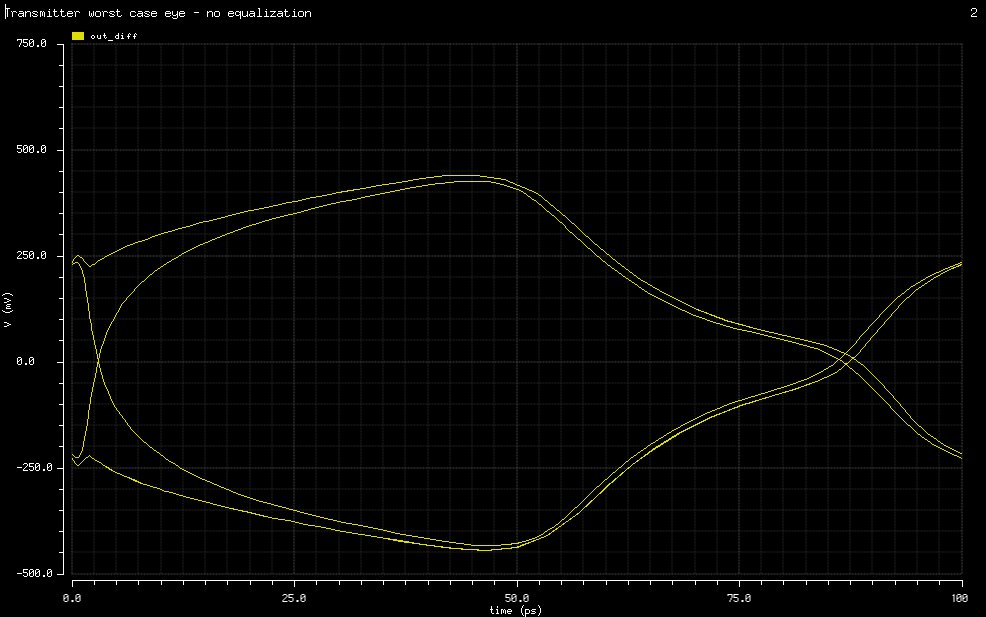
\includegraphics[scale=0.6]{img/wc_eye_no_eq.jpg}}
  \caption{Worst case eye diagram at the transmitter output}
  \label{fig:wc_eye}
\end{figure}

%TODO eye PRBS15, 10,000UI
%TODO wc eye